\documentclass[
   %draft,     % Entwurfsstadium
   final,      % fertiges Dokument
%%%% --- Schriftgröße ---
   10pt,
   %smallheadings,    % kleine Überschriften
   %normalheadings,   % normale Überschriften
   %bigheadings,       % große Überschriften
   headings=big,
%%%% --- Sprache ---
   ngerman,           % wird an andere Pakete weitergereicht
%%%% === Seitengröße ===
   % letterpaper,
   % legalpaper,
   % executivepaper,
   a4paper,
   % a5paper,
   % landscap,
%%%% === Optionen für den Satzspiegel ===
   BCOR5mm,          % Zusaetzlicher Rand auf der Innenseite
   DIV11,            % Seitengroesse (siehe Koma Skript Dokumentation !)
   %DIVcalc,         % automatische Berechnung einer guten Zeilenlaenge
   1.1headlines,     % Zeilenanzahl der Kopfzeilen
   headinclude=false,% Kopf einbeziehen / nicht einbeziehen
   footinclude=false,% Fuss einbeziehen / nicht einbeziehen
   mpinclude=false,  % Margin einbeziehen / nicht einbeziehen
   pagesize,         % Schreibt die Papiergroesse in die Datei.
                     % Wichtig fuer Konvertierungen
%%%% === Layout ===
   oneside,         % einseitiges Layout
   %twoside,          % Seitenraender für zweiseitiges Layout
   %onecolumn,        % Einspaltig
   %twocolumn,       % Zweispaltig
   %openany,         % Kapitel beginnen auf jeder Seite
   %openright,        % Kapitel beginnen immer auf der rechten Seite
                     % (macht nur bei 'twoside' Sinn)
   %cleardoubleplain,    % leere, linke Seite mit Seitenstil 'plain'
   %cleardoubleempty,    % leere, linke Seite mit Seitenstil 'empty'
   titlepage,        % Titel als einzelne Seite ('titlepage' Umgebung)
   %notitlepage,     % Titel in Seite integriert
%%%% --- Absatzeinzug ---
   %                 % Absatzabstand: Einzeilig,
   %parskip,         % Freiraum in letzter Zeile: 1em
   %parskip*,        % Freiraum in letzter Zeile: Viertel einer Zeile
   %parskip+,        % Freiraum in letzter Zeile: Drittel einer Zeile
   %parskip-,        % Freiraum in letzter Zeile: keine Vorkehrungen
   %                 % Absatzabstand: Halbzeilig
   %halfparskip,     % Freiraum in letzter Zeile: 1em
   %halfparskip*,    % Freiraum in letzter Zeile: Viertel einer Zeile
   %halfparskip+,    % Freiraum in letzter Zeile: Drittel einer Zeile
   %halfparskip,     % Freiraum in letzter Zeile: keine Vorkehrungen
   %                 % Absatzabstand: keiner
   %parindent,        % Eingerückt (Standard)
   parskip=true,
%%%% --- Kolumnentitel ---
	 abstracton,			 % Überschrift über den Abstract
   headsepline,      % Linie unter Kolumnentitel
   %headnosepline,   % keine Linie unter Kolumnentitel
   %footsepline,     % Linie unter Fussnote
   %footnosepline,   % keine Linie unter Fussnote
%%%% --- Kapitel ---
   chapterprefix,   % Ausgabe von 'Kapitel:'
   %nochapterprefix,  % keine Ausgabe von 'Kapitel:'
%%%% === Verzeichnisse (TOC, LOF, LOT, BIB) ===
   %listof=totoc,      % Tabellen & Abbildungsverzeichnis ins TOC
   %index=totoc,        % Index ins TOC
   %bibliography=totoc,         % Bibliographie ins TOC
   %bibtotocnumbered, % Bibliographie im TOC nummeriert
   %liststotocnumbered, % Alle Verzeichnisse im TOC nummeriert
   toc=graduated,        % eingereuckte Gliederung
   %tocleft,         % Tabellenartige TOC
   %listof=graduated,      % eingereuckte LOT, LOF
   %listsleft,       % Tabellenartige LOT, LOF
   %pointednumbers,  % Überschriftnummerierung mit Punkt, siehe DUDEN !
   numbers=noenddot, % Überschriftnummerierung ohne Punkt, siehe DUDEN !
   %openbib,         % alternative Formatierung des Literaturverzeichnisses
%%%% === Matheformeln ===
   %leqno,           % Formelnummern links
   fleqn,            % Formeln werden linksbuendig angezeigt
]{scrreprt}
\setlength{\parindent}{0cm} % Absätze nicht einrücken
\setlength{\parskip}{0.65em}
\usepackage[utf8]{inputenc}
\usepackage[ngerman]{babel}
%%% Links ===================================================
\usepackage[
	% Farben fuer die Links
	colorlinks=true,         % Links erhalten Farben statt Kaeten
	urlcolor=pdfurlcolor,    % \href{...}{...} external (URL)
	filecolor=pdffilecolor,  % \href{...} local file
	linkcolor=pdflinkcolor,  %\ref{...} and \pageref{...}
	citecolor=pdfcitecolor,
	% Links
	raiselinks=true,		% calculate real height of the link
	breaklinks,				% Links berstehen Zeilenumbruch
	%backref=page,			% Backlinks im Literaturverzeichnis (section, slide, page, none)
	%pagebackref=true,		% Backlinks im Literaturverzeichnis mit Seitenangabe
	verbose,
	hyperindex=true,		% backlinkex index
	linktocpage=true,		% Inhaltsverzeichnis verlinkt Seiten
	hyperfootnotes=false,	% Keine Links auf Fussnoten
	% Bookmarks
	bookmarks=true,			% Erzeugung von Bookmarks fuer PDF-Viewer
	bookmarksopenlevel=1,	% Gliederungstiefe der Bookmarks
	bookmarksopen=true,		% Expandierte Untermenues in Bookmarks
	bookmarksnumbered=true,	% Nummerierung der Bookmarks
	bookmarkstype=toc,		% Art der Verzeichnisses
	% Anchors
	plainpages=false,		% Anchors even on plain pages ?
	pageanchor=true,		% Pages are linkable
	pdfstartview=Fit,		% Dokument wird Fit Width geaefnet
	pdfpagemode=UseOutlines,	% Bookmarks im Viewer anzeigen
	pdfpagelabels=true,		% set PDF page labels
	pdfpagelayout=SinglePage
]{hyperref}
% ===========================================================

% Laden diverser Pakete======================================
\usepackage{booktabs}
\usepackage{colortbl}
\usepackage{amsmath}
\usepackage{amssymb}
\usepackage{url}
\usepackage{cite}
\usepackage{graphicx}
\usepackage{setspace}
\usepackage{tabularx}
\usepackage{multirow}
\usepackage{xcolor}
\usepackage{tocbasic}
\usepackage{titlesec}
\usepackage{lastpage} 
%\setlength{\textwidth}{14.75cm}
\setlength{\headsep}{1cm}
%\usepackage[top=2.5cm, bottom=4.5cm, headsep=1cm]{geometry}
% ===========================================================



%%% Verweise =============================================================
%
%%% Doc: Documentation inside dtx File
\usepackage[ngerman]{varioref} % Intelligente Querverweise

%-- Einstellungen für VarioRef --
\renewcommand*{\reftextfaceafter}{[siehe \reftextvario{nachfolgende}{kommende}{folgende}{nächste} Seite]} % Verweis auf die nächste Seite
\renewcommand*{\reftextfacebefore}{[siehe \reftextvario{vorherige}{vorhergehende} Seite]} % Verweis auf die vorherige Seite
\renewcommand*{\reftextafter}{\reftextfaceafter}
\renewcommand*{\reftextbefore}{\reftextfacebefore}
\renewcommand*{\reftextcurrent}{[siehe \reftextvario{diese}{aktuelle} Seite]} % Verweis auf derselben Seite
\renewcommand*{\reftextfaraway}[1]{[\reftextvario{siehe auch}{siehe} \reftextvario{Kap.}{Kapitel} \ref{#1} auf \reftextvario{Seite}{S.} \pageref{#1}]} % Verweis auf nicht angrenzende Seite
%\renewcommand*{\vref}[1]{\vpageref{#1}} % Alle Refs nur noch Pageref !!! ansonsten steht Kapitelnummer direkt vor dem eigentlichen VarioRef-Text!!!
\renewcommand*{\vrefrange}[2]{\vpagerefrange{#1}{#2}} % RefRange auf PageRefRange umbiegen, selbes Problem wie vref und vpageref
\newcommand{\vpicref}[1]{Abb. \ref{#1} \vref{#1}}
% ===========================================================



\setcounter{secnumdepth}{2}		% Abbildungsnummerierung mit groesserer Tiefe
\setcounter{tocdepth}{2}		% Inhaltsverzeichnis mit groesserer Tiefe



% Hauptpfade  ===============================================
\graphicspath{{Bilder/}}
\makeatletter
\def\input@path{{content/}}
\makeatother
% ===========================================================


% Kapitel + Nummer + Trennlinie + Name + Trennlinie  ========
\titleformat{\chapter}[display]	% {command}[shape]
  {\usekomafont{chapter}\huge \color{black}}	% format
  {												% label
  \LARGE\MakeUppercase{\chaptertitlename} \Huge \thechapter \filright%
  }%}
  {1pt}										% sep (from chapternumber)
  {\titlerule \vspace{0.9pc} \filright \color{chaptercolor}}    
  %{before}[after] (before chaptertitle and after)
  [\color{black} \vspace{0.9pc} \filright{\titlerule}]

\titleformat*{\section}{\color{sectioncolor}\Large\sffamily}
\titleformat*{\subsection}{\color{sectioncolor}\Large\sffamily}
\titleformat*{\subsubsection}{\color{sectioncolor}\large\sffamily}


%%% Doc: ftp://tug.ctan.org/pub/tex-archive/macros/latex/contrib/caption/caption.pdf
\usepackage{caption}
% Aussehen der Captions
\captionsetup{
   margin = 10pt,
   font = {small,rm},
   labelfont = {small,bf},
   format = plain, % oder 'hang'
   indention = 0em,  % Einruecken der Beschriftung
   labelsep = colon, %period, space, quad, newline
   justification = RaggedRight, % justified, centering
   singlelinecheck = true, % false (true=bei einer Zeile immer zentrieren)
   position = bottom %top
}
% ===========================================================


% Farben ====================================================
% Farbe der Ueberschriften
\definecolor{subsectioncolor}{RGB}{72, 118, 255} % Blau
\definecolor{chaptercolor}{RGB}{0, 0, 130} % Blau (dunkler))
\definecolor{sectioncolor}{RGB}{0, 0, 0}    % Schwarz
%
% Farbe des Textes
\definecolor{textcolor}{RGB}{0, 0, 0}    % Schwarz
%
% Farbe fuer grau hinterlegte Boxen (fuer Paket framed.sty)
\definecolor{shadecolor}{gray}{0.90}

% Farben fuer die Links im PDF
\definecolor{pdfurlcolor}{rgb}{0.6,0,0} % light red
\definecolor{pdffilecolor}{rgb}{0,0.6,0} % bright green
\definecolor{pdflinkcolor}{rgb}{0,0,0.75} % blue
\definecolor{pdfcitecolor}{rgb}{0,0,0} % black

% Farben fuer Listings
\colorlet{stringcolor}{green!40!black!100}
\colorlet{commencolor}{blue!0!black!100}
\definecolor{emphcolor}{rgb}{0,0,0.75}
\definecolor{lightgray}{rgb}{.9, .9, .9}
\definecolor{blue}{RGB}{58,95,205}
\definecolor{black}{RGB}{0, 0, 0}
\definecolor{darkgray}{rgb}{.4,.4,.4}
% ===========================================================


% Codelisting ===============================================
\usepackage{listings}
\lstset{
  numbers=left,               % Ort der Zeilennummern
  numberstyle=\tiny,          % Stil der Zeilennummern
  stepnumber=2,               % Abstand zwischen den Zeilennummern
  numbersep=-5pt,             % Abstand der Nummern zum Text
  tabsize=2,                  % Groesse von Tabs
  extendedchars=true,         %
  breaklines=true,            % Zeilen werden Umgebrochen
  stringstyle=\color{stringcolor}, % Farbe der String
	keywordstyle=\bfseries\color{violet},
	ndkeywordstyle=\bfseries\color{blue},
	commentstyle=\itshape\color{darkgray},
	emphstyle=\color{red},
	basicstyle=\small\ttfamily\color{black}\singlespacing, % Standardschrift
  showspaces=false,			% Leerzeichen anzeigen ?
  showtabs=false,			% Tabs anzeigen ?
  showstringspaces=false,	% Leerzeichen in Strings anzeigen ?
  frame=tlrb,				% Rahmen um das Listing (Großbuchstaben = doppelt)
  captionpos=b,						% Position der Caption (t|b)
	belowcaptionskip=\medskipamount,	%Platz unter der Caption
	aboveskip=\medskipamount,		% Platz über dem Listing
	backgroundcolor=\color{lightgray}, % Hintergrundfarbe der Box
	numberbychapter=true,			% Nummerierung der Listings nach den Kapiteln
	rulesepcolor=\color{white},		% Farbe des Hintergrunds zwischen innerem und äußerem Rahmen
	rulesep=0pt,						% Abstand der Rahmen voneinander
	%framexleftmargin=2mm,			% Box nach links erweitern
	firstnumber=1,					% Beginne mit 1 als Zeilennummer
	escapechar=\#
 }

\lstdefinelanguage{JavaScript}{
  keywords={typeof, new, true, false, catch, function, return, null, catch, switch, var, if, in, while, do, else, case, break},
  ndkeywords={class, export, boolean, throw, implements, import, this},
  sensitive=false,
  comment=[l]{//},
  morecomment=[s]{/*}{*/},
  morestring=[b]',
  morestring=[b]"
}

\lstdefinelanguage{Franca}{
  keywords={package, typeCollection, interface, attribute, is, method, version},
  ndkeywords={enumeration, typedef, struct, array, in, out, String, Float, Int8, Int16, Int32, Int64, UInt8, UInt16, UInt32, UInt64, major, minor},
  sensitive=false,
  comment=[l]{//},
  morecomment=[s]{<**}{**>},
  morestring=[b]',
  morestring=[b]"
}

\lstdefinelanguage{C++}{
  keywords={typeof, new, true, false, catch, function, return, null, catch, switch, var, if, in, while, do, else, case, break},
  ndkeywords={class, export, boolean, throw, implements, import, this, auto, int},
  sensitive=false,
  comment=[l]{//},
  morecomment=[s]{/*}{*/},
  morestring=[b]',
  morestring=[b]"
}

\lstdefinelanguage{XML}{
  keywords={DOCTYPE, PUBLIC, ELEMENT, ATTLIST, xml, REQUIRED},
  alsoletter={:,-},
  morekeywords={xsl:stylesheet, xsl:template, xsl:applytemplates, xsl:value-of, xsl:apply-templates, xsl:for-each, xsl:if, xsl:variable, xsl:choose, xsl:when, xsl:otherwise, xsl:sort, xsl:call-template, xsl:attribute},
  ndkeywords={version, select, match, name},
  sensitive=false,
  comment=[s]{!--}{--},
  morecomment=[s]{<?}{?>},
  morestring=[s]{>}{<},
  morestring=[b]',
  morestring=[b]"
}

\lstdefinelanguage{SVG}{
  keywords={DOCTYPE, PUBLIC, ELEMENT, ATTLIST, xml, REQUIRED},
  alsoletter={:,-},
  morekeywords={line, circle, rect, ellipse, polyline, polygon},
  ndkeywords={width, height, x, x1, x2, y, y1, y2, cx, cy, r, rx, ry, points},
  sensitive=false,
  comment=[s]{!--}{--},
  morecomment=[s]{<?}{?>},
  morestring=[s]{>}{<},
  morestring=[b]',
  morestring=[b]"
}

\lstloadlanguages{XML, HTML, C++, JavaScript}
% ===========================================================

%
\usepackage{fancyhdr}
%Einstelllungen Kopfzeile
\fancyhead[L]{}
%\renewcommand{\headrulewidth}{0.0pt} %obere Trennlinie entfernt

\setlength{\intextsep}{1.5\baselineskip} % Platz ober- und unterhalb des Bildes

%Einstellungen Fußzeile
\fancyfoot[L]{\textsf{Jan Ulses}}
\fancyfoot[C]{}
\fancyfoot[R]{\textsf{Seite {\thepage} von \pageref{LastPage}}}

\title{Test und Validierung von generiertem Middleware Sourcecode}
\author{Jan Ulses}
\date{15. September 2014}

\setkomafont{captionlabel}{\sffamily}

% Hurenkinder und Schusterjungen verhindern
\clubpenalty=10000
\widowpenalty=10000
\displaywidowpenalty=10000
%%%%%

\usepackage[german=quotes]{csquotes}

\begin{document}

%%%%% Titelseite
\begin{titlepage}

  \onehalfspacing
  \begin{figure}[htbp]
    \begin{minipage}{0.4\textwidth}
     \centering
      
\includegraphics[width=5cm]{DHBW-Logo.png}
    \end{minipage}\hfill
    \begin{minipage}{0.4\textwidth}
     \centering
      
\includegraphics[width=5cm]{Harman-Logo.jpg}
    \end{minipage}
  \end{figure}

  \begin{center}	
	\vspace*{3cm}
    \huge \textbf{Bussysteme\\}
	%\noindent\rule{12cm}{0.4pt}\\
	\vspace*{2cm}
    \Large Vorlesungsmitschrieb\\
    \vspace*{0,75cm}
    \normalsize des Studiengangs\\
    \Large Informationstechnik\\
    \vspace*{1cm}
    \normalsize von\\
    \Large Jan Ulses\\
    \vspace*{1cm}
    \large \today\\
    \vspace*{2cm}
    \small
    \renewcommand{\arraystretch}{1,2}
    \singlespacing
    \begin{tabular}{rcl}
    	\hline
  		Dozent: & & Jürgen Röthig\\
  		E-Mail: & & jr@roethig.de\\
  		Vorlesungszeitraum: & \hspace*{0,5mm} & 09.02.15 - 10.05.15 \\
  		Klausurtermin: & & 04.05.2015\\
  		Autor: & & Jan Ulses\\
  		Kurs: & & TINF12B3\\
  		Ausbildungsfirma: & & Harman/Becker Automotive Systems GmbH\\
  		Studiengangsleiter: & & Jürgen Vollmer\\
  		\hline
 	\end{tabular}
    
  \end{center}
  \normalsize
  \vfill
  
\end{titlepage}
\pagenumbering{Roman}
\onehalfspacing
% ==============================================

%%%%% Abbildungsverzeichnis
\listoffigures
\addcontentsline{toc}{chapter}{\protect\numberline{}{Abbildungsverzeichnis}} % Nicht nummerierter TOC Eintrag
\newpage
% ==============================================

%%%%% Tabellenverzeichnis
\listoftables
\addcontentsline{toc}{chapter}{\protect\numberline{}{Tabellenverzeichnis}} % Nicht nummerierter TOC Eintrag
\newpage
% ==============================================

%%%%% Listings
%\lstlistoflistings
%\addcontentsline{toc}{chapter}{\protect\numberline{}{Listings}} % Nicht nummerierter TOC Eintrag
% ==============================================

%%%%% Vorwort
% ==============================================
\chapter*{Vorwort}
\addcontentsline{toc}{chapter}{\protect\numberline{}{Vorwort}} % Nicht nummerierter TOC Eintrag
Dieser Vorlesungsmitschrieb ist im 6.Semester des Studiengangs Informationstechnik an der DHBW-Karlsruhe entstanden und wurde mit \LaTeX verfasst. Die Quelldateien sind \href{https://github.com/julses/Bussysteme}{hier} in einem GIT-Repository zu finden.
\par
Das Fach Bussysteme behandelt das Thema eines Datenbus. Dieser überträgt Daten zwischen Computerbestandteilen innerhalb eines Computers oder zwischen verschiedenen Computern. Anders als bei einem Anschluss, bei dem ein Gerät mit einem anderen Gerät über eine oder mehrere Leitungen verbunden ist, kann ein Bus mehrere Peripheriegeräte über den gleichen Satz von Leitungen miteinander verbinden.
\par
Besonderer Dank geht an meinen Arbeitskollegen Sascha Moser, der hier für Grafiken und Anpassungen des Mitschriebs ausgeholfen hat.\\
Ein Dank geht auch an die Kommilitonen, welche in jeder Vorlesung ein Vorlesungsmitschrieb auf Google-Docs aktualisiert haben. Dieses konnte wunderbar bei Vorlesungsversäumnissen zum Nachtragen in dieses Dokument genutzt werden und kann \href{https://www.google.com/url?q=https%3A%2F%2Fdocs.google.com%2Fdocument%2Fd%2F1bVH2fVSst7iG3dhWXjIo6FsLtSjdwrZTV5Z2JXYnOfI%2Fedit%3Fusp%3Dsharing}{hier} eingesehen werden.
\begin{figure}[htbp]
  \centering
  
\includegraphics[width=4.5cm]{vorwort.png}
\end{figure}
\newpage
% ==============================================

%%%%% Inhaltsverzeichnis
\tableofcontents
\newpage
\pagestyle{fancy}
\pagenumbering{arabic}
% ==============================================
\setcounter{page}{5}

%%%%% Hauptteil
% ==============================================
\chapter{Grundlagen}



% Wortherkunft ====================================
\section{Wortherkunft}
\label{sec:wortherkunft}

\begin{description}
\item[Bus] „omnibus“ lat. „für alle“
\item[hier:] Kommunikationsmedium „für alle“
\item[klass. „shared medium“:] Was einer der Teilnehmer auf dem Medium sendet, hören (potentiell) alle Teilnehmer gleichzeitig mit.
\end{description}
% =================================================



% Topologien ======================================
\section{Topologien von „Computernetzen“}
\label{sec:topologien}

\subsubsection{Stern}
\begin{figure}[htbp]
  \centering
  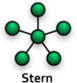
\includegraphics[scale=1]{Stern-Topologie.png}
  \caption{Stern-Topologie}
\end{figure}
Es gibt einen zentralen „Sternverteiler“ in der Mitte und dedizierte Leitungen von diesem zu jedem der Teilnehmer. Üblicherweise ist der Sternverteiler \underline{nicht} auch ein „normaler Teilnehmer“.\\

\subsubsection{Ring}
\begin{figure}[htbp]
  \centering
  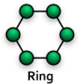
\includegraphics[scale=1]{Ring-Topologie.png}
  \caption{Ring-Topologie}
\end{figure}
Jeder Teilnehmer hat genau einen Vorgänger und einen Nachfolger, mit denen er jeweils verbunden ist.

\subsubsection{Bus}
\begin{figure}[htbp]
  \centering
  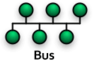
\includegraphics[scale=1]{Bus-Topologie.png}
  \caption{Bus-Topologie}
\end{figure}
Es gibt lediglich eine „Leitung“ als „shared medium“, mit welchem jeder Teilnehmer über eine „Stichleitung“ verbunden ist.

\subsubsection{Maschennetz}
\begin{figure}[htbp]
  \centering
  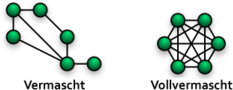
\includegraphics[scale=1]{Vermascht-Topologie.png}
  \caption{Maschen-Topologie}
\end{figure}
Jeder Teilnehmer hat zu beliebig vielen anderen Teilnehmern jeweils eine dedizierte Verbindung. Beim Spezialfall Vollvermascht hat jeder Teilnhemer eine Verbindung zu demem anderen Teilnehmer.

\subsubsection{Baum}
\begin{figure}[htbp]
  \centering
  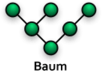
\includegraphics[scale=1]{Baum-Topologie.png}
  \caption{Baum-Topologie}
\end{figure}
Die Baumtopologie ist eine hierarchische Topologie. Ausgehend von einem „Wurzel Teilnehmer“ gibt es jeweils ein oder mehrere Verbindungen zu Teilnehmern der nächsten Hierarchieebene.

\subsubsection{Linie}
\begin{figure}[htbp]
  \centering
  
\includegraphics[scale=1]{Linie-Topologie.png}
  \caption{Linien-Topologie}
\end{figure}
Jeder Teilnehmer ist mit maximal zwei Teilnehmern verbunden. Es gibt einen Anfang und ein Ende.
% =================================================



% Bustopologie ====================================
\section{Verwenden alle „Bussysteme“ eine Bustopologie?}
\begin{table}[h]
\centering
\begin{tabular}{c|c}
\textbf{Bustopologie} & \textbf{Bustopologie} \\ 
\hline 
Ethernet in BNC-Verkabelung & USB: Baum \\ 
\hline 
ProfiBus & MOST: Ring \\ 
\hline 
WLAN & Ethernet in TP-Verkabelung: Baum \\ 
\hline
IDE (P-Data) & (S-ATA)\\
\hline
PCI & (PCI-Express)\\
\hline
SCSI & (SAS (Seriell Attached SCSI))\\
\hline
 & Firewire: vermaschtes Netz\\
 & mit Einschränkungen
\end{tabular}
\caption{Einordnung von Technologien in Bussysteme}
\label{tab:bussystem_or_not}
\end{table} 
Viele der heutigen „Bussysteme“ sind physikalisch keine \underline{Busse}, sondern nur noch logisch/protokolltechnisch auf einer höheren Ebene.
% =================================================



% Spezielle Aufgaben von Bussystemen ==============
\section{Spezielle Aufgaben von Bussystemen}
\label{sec:spezielle_Aufgaben_Bussysteme}
Speziell bei Bussystemen zu lösende Aufgaben:
\begin{itemize}
\item Medienzugriff
\item Adressierung
\end{itemize}
% =================================================
\newpage
% ==============================================
%\include{content/02-ausgewaehlte_Bussysteme}
	%Busse der Informationstechnik
	%Feldbusse
%\newpage
% ==============================================

%\pagenumbering{Roman}
%\setcounter{page}{5}

\end{document}